Apart from zero-shot image-text matching, we perform more experiments on Winoground to explore \textbf{synthetic dataset generation}. As we have seen in the previous section models perform badly in Winoground. The problem is that only zero-shot can be done because Winoground has no training data. Annotating examples for Winoground is very time-consuming and therefore creating a big dataset for training is very difficult. Therefore, compositional reasoning has to be learned either in pretraining or when fine-tuning with other datasets. However, there is no training dataset that focuses on compositional reasoning. A solution could be to create a synthetic dataset for compositional reasoning and fine-tune the models with it.

We explore three different options for synthetic dataset generation. These options are Text-to-Image Generation (\ref{sec:text_to_image_generation}), Image Captioning (\ref{sec:image_captioning}) and Image Retrieval (\ref{sec:image_retrieval}). These experiments also allow us to gain more insight into the dataset and the tested models.

\section{Text-to-Image Generation} \label{sec:text_to_image_generation}

As noted, large generative \textbf{text-to-image diffusion models}, like DALLE-2 \cite{ramesh2022hierarchical} and IMAGEN \cite{saharia2022photorealistic}, are able to generate stunning images. They are known to possess some visual-reasoning skills \cite{cho2022dall}. However, a recent work \cite{liu2022compositional} has shown that they \textbf{struggle to understand the composition of some concepts}, such as confusing the attributes and relations of different objects. Here we want to know if they are good enough for synthetic dataset generation.

\subsection{Automatic Generation}

With the aim of evaluating the compositional ability of diffusion models, we used the state-of-the-art Stable Diffusion model \cite{rombach2021highresolution} to generate images from Winoground captions. We generate images 9 images for each Winoground caption, which results in a total of $800*9=7200$ images. We do a qualitative evaluation of the generated images. Here we will have a look at a few examples of generated images to compare them with the original images. We select the same captions that were used to present the Winoground dataset in the previous section. Only the first generated image is shown in the examples, which is not necessarily the best one.

In \cref{fig:stable-diffusion-examples}, there are both correct and incorrect images. The first image in the first pair is correct, but the second one is wrong. The colour of the dog is correct in the next image, but the colour of the couch is mistaken. Finally, the last two images are wrong, food is missing in the first image and the shape is wrong in the second.

\begin{figure}[ht]
\centering
    \begin{minipage}[t]{.30\textwidth}
        \begin{subfigure}[t]{\textwidth}
        \centering
        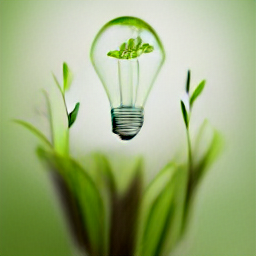
\includegraphics[height=4cm]{stable_diffusion/ex_155_cap_0_img_0.png}
        \caption{[some plants] surrounding [a lightbulb]}
        \end{subfigure}\\
        \begin{subfigure}[t]{\textwidth}
        \centering
        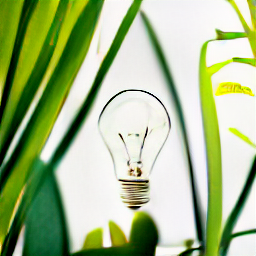
\includegraphics[height=4cm]{stable_diffusion/ex_155_cap_1_img_0.png}
        \caption{[a lightbulb] surrounding [some plants]}
        \end{subfigure}%
        \caption*{\textit{Object}}
    \end{minipage}
    \hfill
    \begin{minipage}[t]{.30\textwidth}
        \begin{subfigure}[t]{\textwidth}
        \centering
        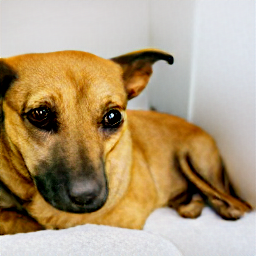
\includegraphics[height=4cm]{stable_diffusion/ex_29_cap_0_img_0.png}
        \caption{a [brown] dog is on a [white] couch}
        \end{subfigure}\\
        \vspace{10pt}
        \begin{subfigure}[t]{\textwidth}
        \centering
        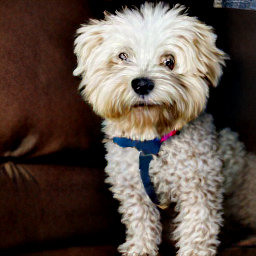
\includegraphics[height=4cm]{stable_diffusion/ex_29_cap_1_img_0.png}
        \caption{a [white] dog is on a [brown] couch}
        \end{subfigure}%
        \vspace{10pt}
        \caption*{\textit{Relation}}
    \end{minipage}
    \hfill
    \begin{minipage}[t]{.30\textwidth}
        \begin{subfigure}[t]{\textwidth}
        \centering
        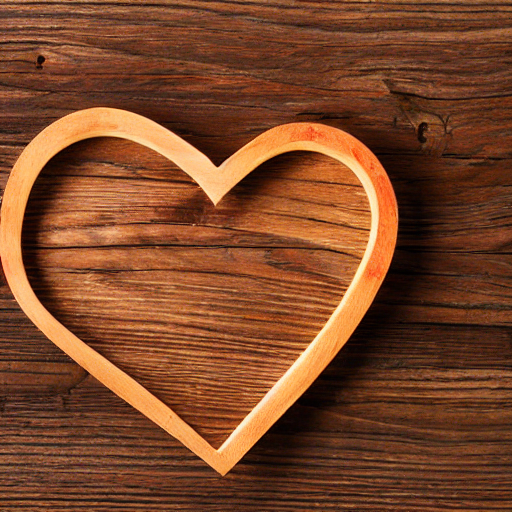
\includegraphics[height=4cm]{stable_diffusion/ex_118_cap_0_img_0.png}
        \caption{[circular] food on [heart-shaped] wood}
        \end{subfigure}\\
        \begin{subfigure}[t]{\textwidth}
        \centering
        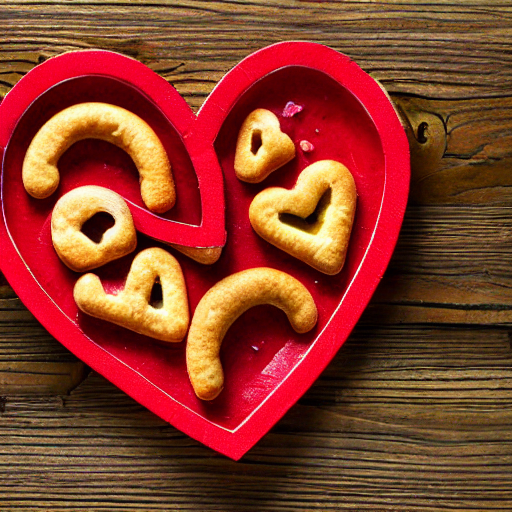
\includegraphics[height=4cm]{stable_diffusion/ex_118_cap_1_img_0.png}
        \caption{[heart-shaped] food on [circular] wood}
        \end{subfigure}%
        \caption*{\textit{Relation}}
    \end{minipage}%
    \caption{Stable Diffusion examples for the swap-dependent linguistic tags \textit{Object}, \textit{Relation} and \textit{Relation} from left to right. The linguistic examples are additionally tagged with 1 main predicate.}
    \label{fig:stable-diffusion-examples}
\end{figure}

In \cref{fig:stable-diffusion-examples-linguistic}, both images of the first pair correspond to the first caption. In the second pair, both images correspond to the second caption. The third pair is the only one that is completely correct.

\begin{figure}[ht]
\centering
    \begin{minipage}[t]{.30\textwidth}
        \begin{subfigure}[t]{\textwidth}
        \centering
        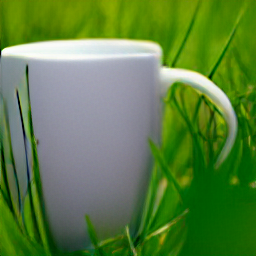
\includegraphics[height=4cm]{stable_diffusion/ex_14_cap_0_img_0.png}
        \caption{there is [a mug] in [some grass]}
        \end{subfigure}\\
        \begin{subfigure}[t]{\textwidth}
        \centering
        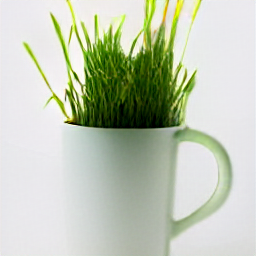
\includegraphics[height=4cm]{stable_diffusion/ex_14_cap_1_img_0.png}
        \caption{there is [some grass] in [a mug]}
        \end{subfigure}%    
        \caption*{\textit{Object}}
    \end{minipage}
    \hfill
    \begin{minipage}[t]{.30\textwidth}
        \begin{subfigure}[t]{\textwidth}
        \centering
        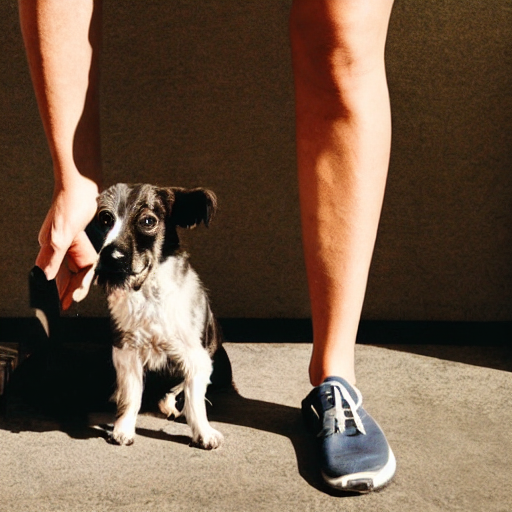
\includegraphics[height=4cm]{stable_diffusion/ex_21_cap_0_img_0.png}
        \caption{a person [sits] and a dog [stands]}
        \end{subfigure}\\
        \begin{subfigure}[t]{\textwidth}
        \centering
        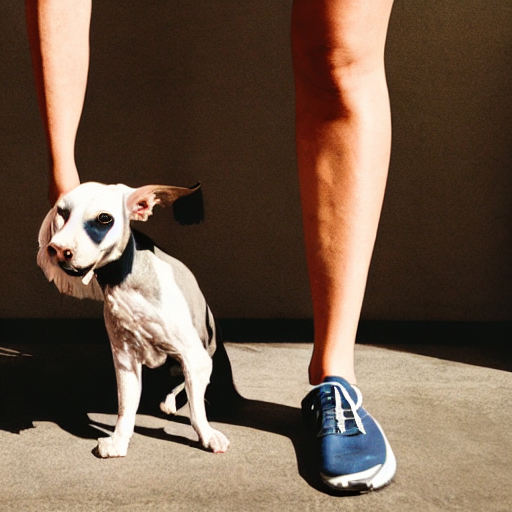
\includegraphics[height=4cm]{stable_diffusion/ex_21_cap_1_img_0.png}
        \caption{a person [stands] and a dog [sits]}
        \end{subfigure}%    
        \caption*{\textit{Relation}}
    \end{minipage}
    \hfill
    \begin{minipage}[t]{.30\textwidth}
        \begin{subfigure}[t]{\textwidth}
        \centering
        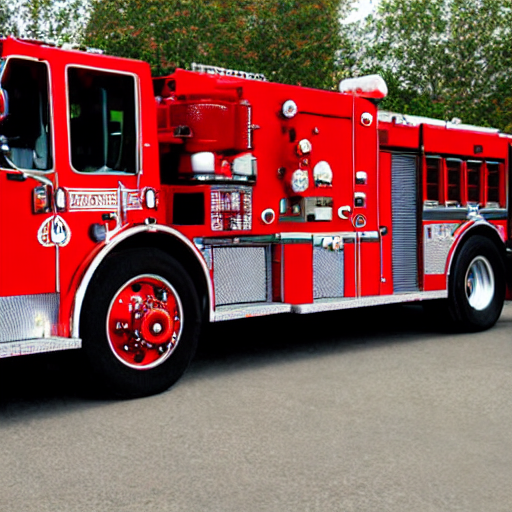
\includegraphics[height=4cm]{stable_diffusion/ex_72_cap_0_img_0.png}
        \caption{it's a [fire] [truck]}
        \end{subfigure}\\
        \begin{subfigure}[t]{\textwidth}
        \centering
        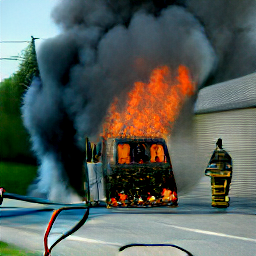
\includegraphics[height=4cm]{stable_diffusion/ex_72_cap_1_img_0.png}
        \caption{it's a [truck] [fire]}
        \end{subfigure}%
        \caption*{\textit{Both}}
    \end{minipage}%
    \caption{Stable Diffusion examples for the swap-dependent linguistic tags \textit{Object}, \textit{Relation} and \textit{Both} from left to right. The linguistic examples are additionally tagged with 1, 2 and 1 main predicates from left to right.}
    \label{fig:stable-diffusion-examples-linguistic}
\end{figure}

In \cref{fig:stable-diffusion-examples-visual}, both examples in the first image are wrong, there is no magnifying glass. In the second pair, only the person with the ponytail is shown. The last pair only has three windows, there is no people in neither of them.

\begin{figure}[ht]
\centering
    \begin{minipage}{.30\textwidth}
        \begin{subfigure}{\textwidth}
        \centering
        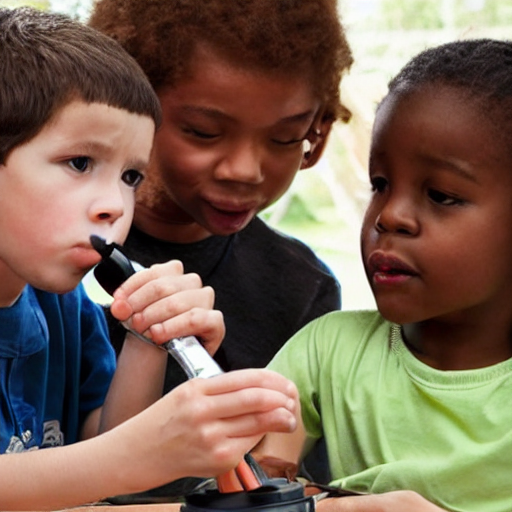
\includegraphics[height=4cm]{stable_diffusion/ex_75_cap_0_img_0.png}
        \caption{the kid [with the magnifying glass] looks at them []}
        \end{subfigure}\\
        \begin{subfigure}{\textwidth}
        \centering
        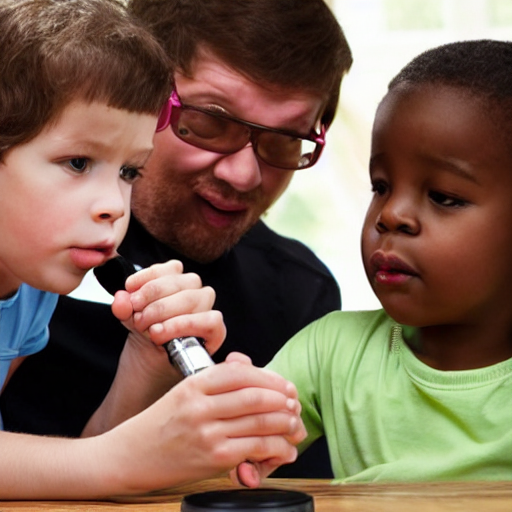
\includegraphics[height=4cm]{stable_diffusion/ex_75_cap_1_img_0.png}
        \caption{the kid [] looks at them [with the magnifying glass]}
        \end{subfigure}%    
        \caption*{\textit{Pragmatics}}
    \end{minipage}
    \hfill
    \begin{minipage}{.30\textwidth}
        \begin{subfigure}{\textwidth}
        \centering
        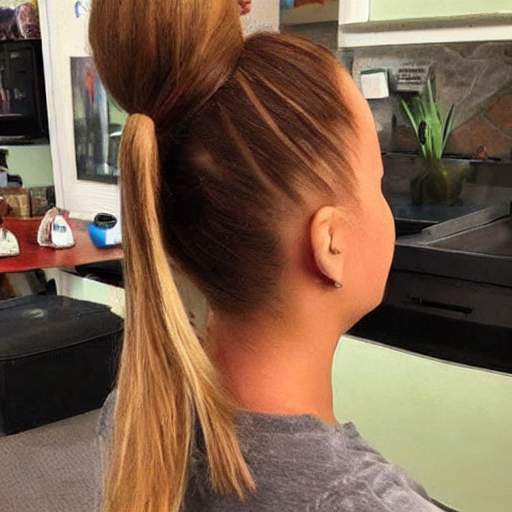
\includegraphics[height=4cm]{stable_diffusion/ex_27_cap_0_img_0.png}
        \caption{the person with the ponytail [packs] stuff and other [buys] it}
        \end{subfigure}\\
        \begin{subfigure}{\textwidth}
        \centering
        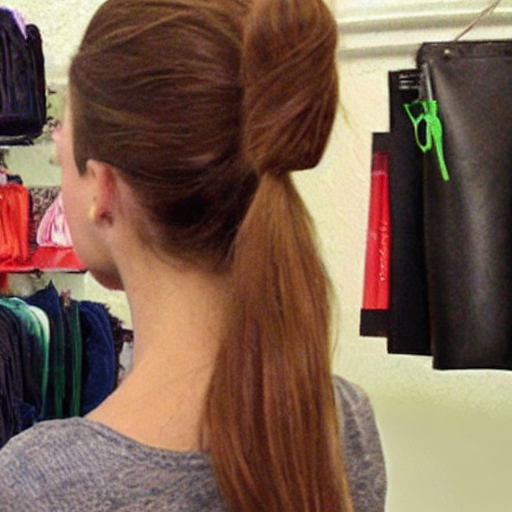
\includegraphics[height=4cm]{stable_diffusion/ex_27_cap_1_img_0.png}
        \caption{the person with the ponytail [buys] stuff and other [packs] it}
        \end{subfigure}%    
        \caption*{\textit{Series}}
    \end{minipage}
    \hfill
    \begin{minipage}{.30\textwidth}
        \begin{subfigure}{\textwidth}
        \centering
        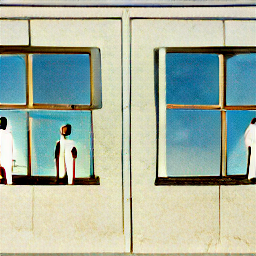
\includegraphics[height=4cm]{stable_diffusion/ex_61_cap_0_img_0.png}
        \caption{there are [three] people and [two] windows}
        \end{subfigure}\\
        \begin{subfigure}{\textwidth}
        \centering
        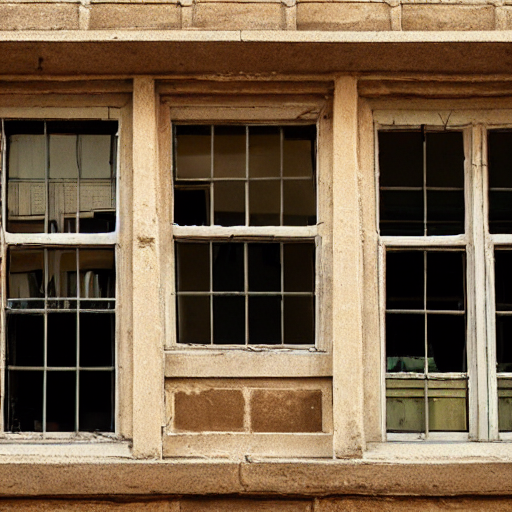
\includegraphics[height=4cm]{stable_diffusion/ex_61_cap_1_img_0.png}
        \caption{there are [two] people and [three] windows}
        \end{subfigure}%    
        \caption*{\textit{Symbolic}}
    \end{minipage}
    \caption{Stable Diffusion examples for the visual tags \textit{Pragmatics}, \textit{Series} and \textit{Symbolic} from left to right. The visual examples are additionally tagged with the \textit{Relation} tag, and 1, 2, and 1 main predicates from left to right.}
    \label{fig:stable-diffusion-examples-visual}
\end{figure}

\subsection{Manual Evaluation}

We used Label Studio \cite{labelstudio} to annotate images generated by Stable Diffusion. As annotating all the images would take a very long time, we choose to annotate a subset of examples, and only one image per caption. 

In each annotation there are two captions from Winoground and two images generated with Stable Diffusion. Each image is created from one caption but the order of the images is random. The annotators have to choose which text corresponds to each image: the first caption, the second caption, both or none. An screenshot of the annotation interface can be seen in \cref{fig:label-studio-annotation}.

\begin{figure}[ht]
    \centering
    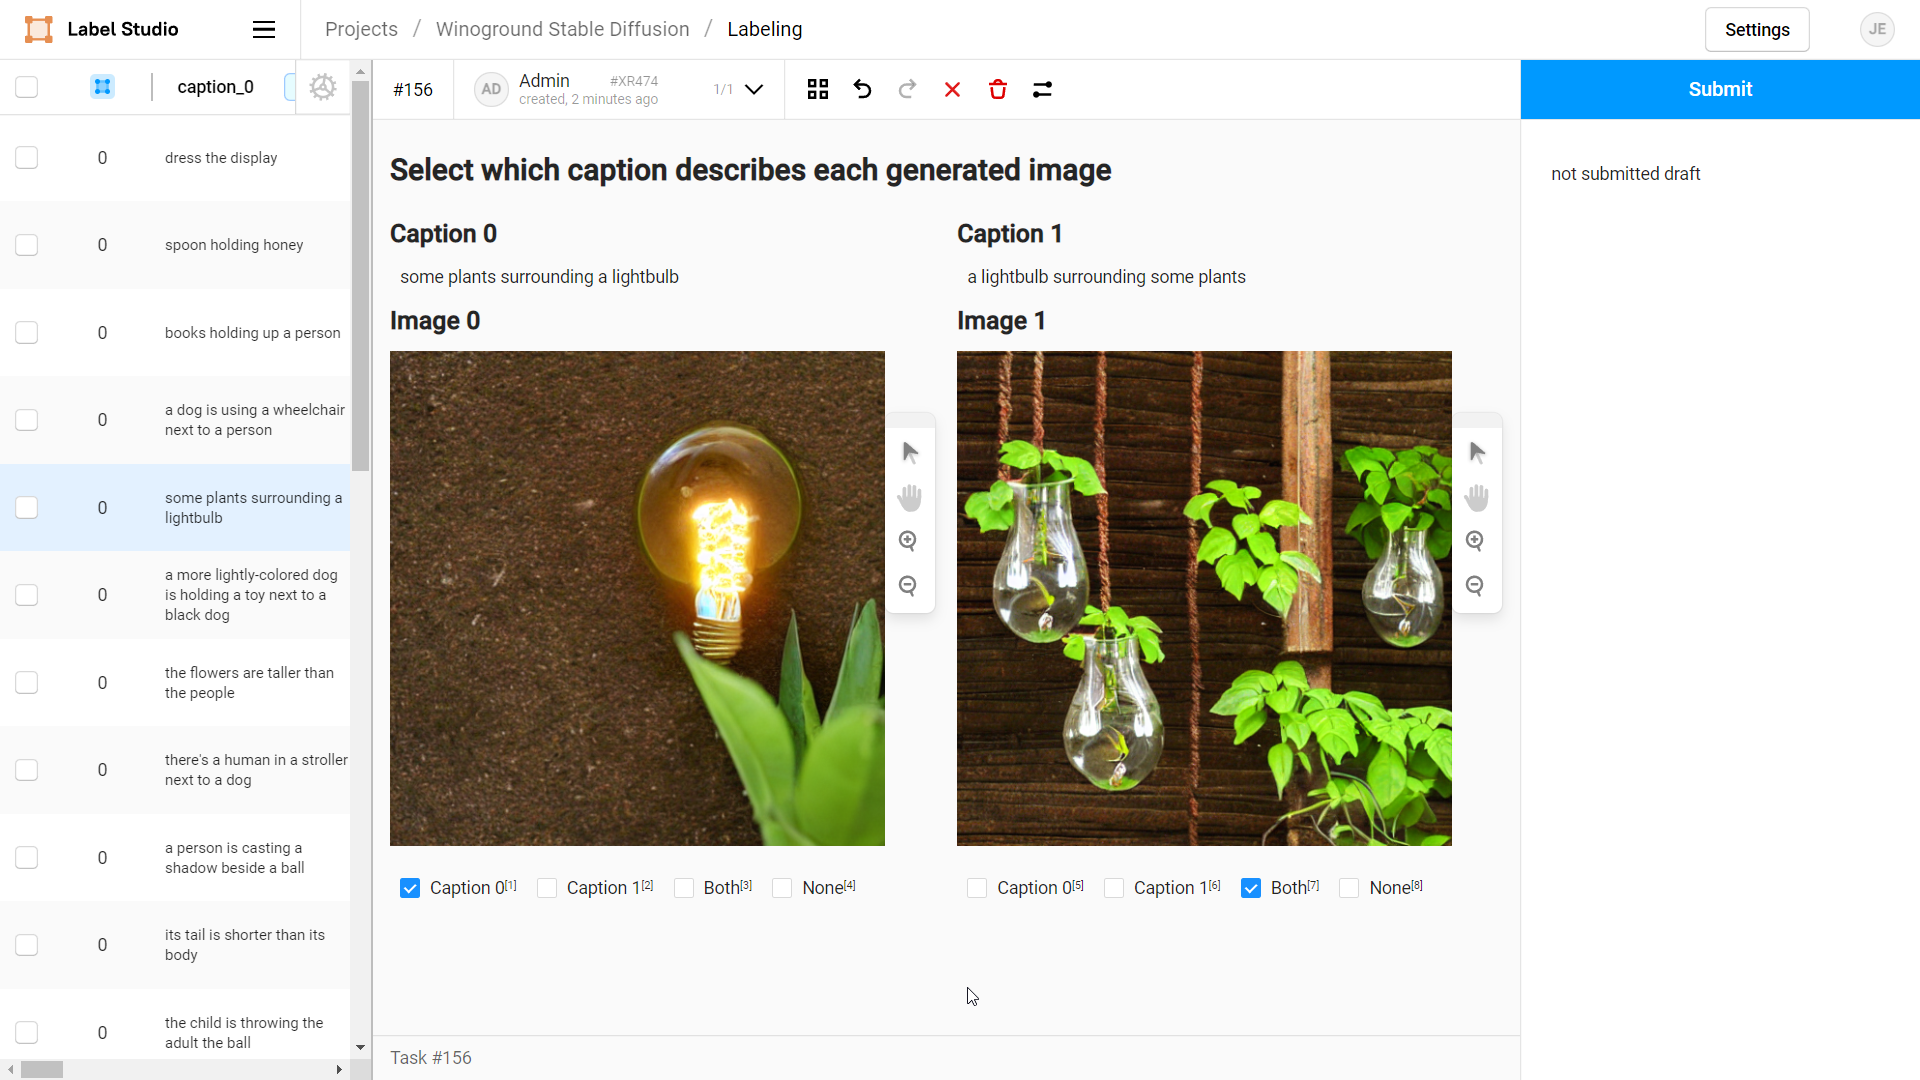
\includegraphics[width=\linewidth]{images/annotation/label-studio-annotation.png}
    \caption{Label Studio annotation interface}
    \label{fig:label-studio-annotation}
\end{figure}

There were 6 annotators in total and each one annotated 50 examples, for a total of 300 annotated examples. Each example includes two images, for a total of 600 annotated images. There are 400 examples in total, so we decided that it is a big enough subset.

The statistics of the annotation task are shown in \cref{tab:annotation}. The general conclusion is that Stable Diffusion is not good at this task. Most of the images do not match any of the captions, 351 out of 600. There are only 25 images that match both captions. The remaining images match one caption or the other (224), but there are many that match the incorrect caption (94). If we take into account image pairs, there are only a few correct ones, 23 out of 300.

\begin{table}[ht]
    \centering
    \begin{tabular}{l|rrrr|r}
    \toprule
    {} & Caption 0  &  Caption 1 &  Both &  None & All \\
    \midrule
    Caption 0    &   65 &  48 &  12 & 175 & 300\\
    Caption 1    &   46 &  65 &  13 & 176 & 300\\
    \midrule
    All  &   111 &    113 &    25 &    351 & 600\\
    \bottomrule
    \end{tabular}
    \caption{Statistics of the annotations. Rows shows the caption used for generation and columns show the annotation choice.}
    \label{tab:annotation}
\end{table}

Therefore, using a diffusion model for data augmentation might not be robust enough. It would require generating many images to get correct ones, and manual filtering to discard the wrong images. In \cref{sec:image_retrieval}, we will test another approach to obtain similar images. Instead of generating new images, they are retrieved from a huge dataset.

\section{Image Captioning} \label{sec:image_captioning}

With the aim of obtaining more insight about the Winoground examples, we decided to test image captioning. We used OFA \cite{wang2022unifying} and BLIP \cite{li2022blip} models of different sizes to generate captions for all Winoground images. To run BLIP models, we used LAVIS: A Library for Language-Vision Intelligence \cite{li2022lavis}. We chose these models because they are SOTA in image captioning and we also use them in other evaluations. Our intention was to compare them with the real captions. We calculated BLEU scores for all models and we found out that they are very low (see \cref{tab:bleu_scores}). This indicates that the captions generated by these models are very far from the real captions.

\begin{table}[ht]
    \centering
    \begin{tabular}{lrrrr}
    \toprule
    Model &  BLEU-1 &  BLEU-2 &  BLEU-3 &  BLEU-4 \\
    \midrule
    OFA$_{Tiny}$    &   14.40 &    5.76 &    2.50 &    1.30 \\
    OFA$_{Base}$    &   16.68 &    7.12 &    3.26 &    1.58 \\
    OFA$_{Medium}$  &   16.28 &    6.47 &    2.84 &    1.39 \\
    OFA$_{Large}$   &   15.10 &    6.45 &    3.03 &    1.53 \\
    OFA$_{Huge}$    &   15.73 &    6.94 &    3.06 &    1.35 \\
    BLIP (ViT-B/16) &   17.80 &    8.10 &    3.96 &    2.01 \\
    BLIP (ViT-L/16) &   17.96 &    8.31 &    4.36 &    2.50 \\
    \bottomrule
    \end{tabular}
    \caption{Image captioning BLEU scores of OFA and BLIP models.}
    \label{tab:bleu_scores}
\end{table}

One reason for this could be that the real Winoground captions are not typical captions. They are hand-crafted so that they contain the same words in a different order, and that conditions the captions. Another reason could be that these models are not good at describing these types of images that require compositional reasoning. As these models are not very good at matching Winoground images with captions.

Analysing the captions manually would be necessary to know how good they really are. We show some caption examples of the best performing model, BLIP large, so that we can compare them with the original ones. The complete caption files for all the models can be found in the GitHub repository.

In \cref{fig:captioning-examples}, all the captions are correct. They describe the images correctly. Some descriptions are more detailed that in the original captions, but some attributes are also missing. For example, the color of the couch and the shape of the cutting wood are not mentioned.

\begin{figure}[ht]
\centering
    \begin{minipage}[t]{.30\textwidth}
        \begin{subfigure}[t]{\textwidth}
        \centering
        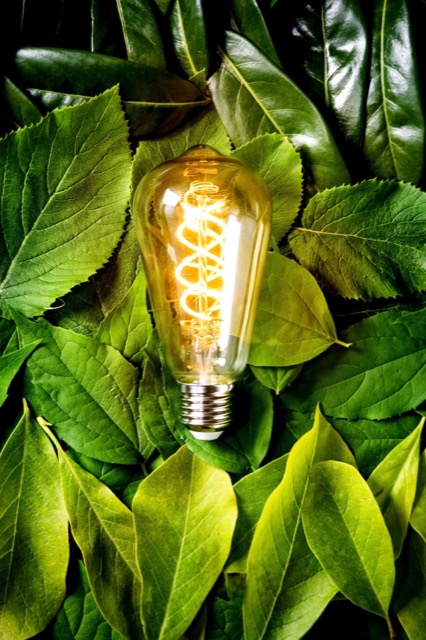
\includegraphics[height=3cm]{ex_155_img_0.png}
        \caption{a light bulb sitting on top of a pile of green leaves}
        \end{subfigure}\\
        \begin{subfigure}[t]{\textwidth}
        \centering
        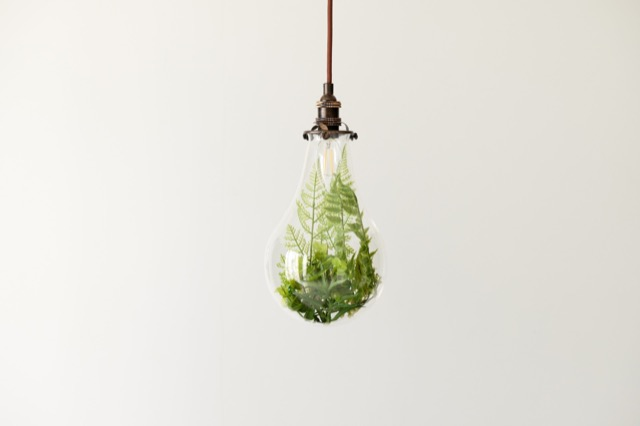
\includegraphics[height=3cm]{ex_155_img_1.png}
        \caption{a light bulb with a plant inside of it}
        \end{subfigure}%
        \caption*{\textit{Object}}
    \end{minipage}
    \hfill
    \begin{minipage}[t]{.30\textwidth}
        \begin{subfigure}[t]{\textwidth}
        \centering
        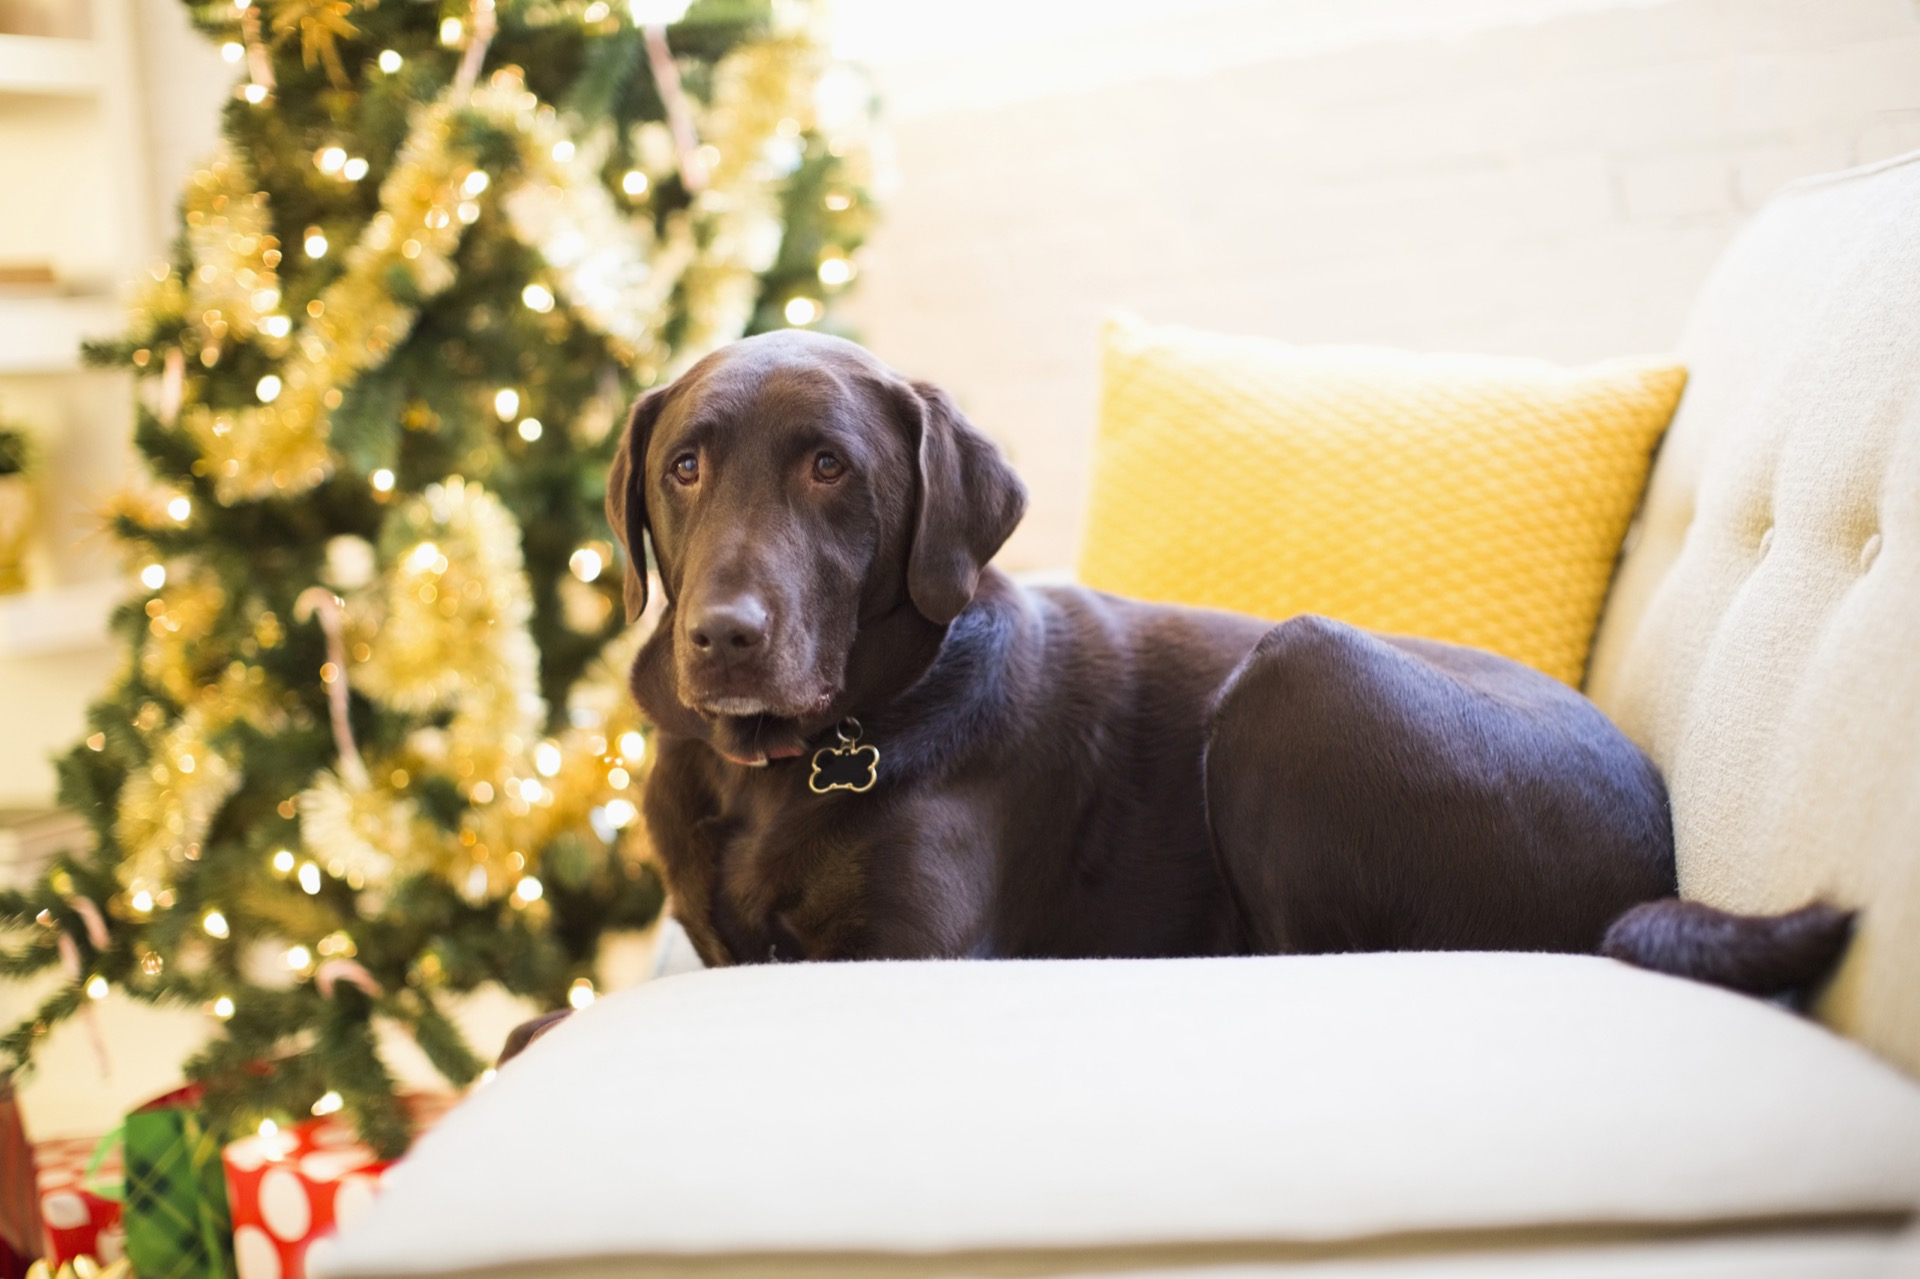
\includegraphics[height=3cm]{ex_29_img_0.png}
        \caption{a black dog sitting on a couch in front of a christmas tree}
        \end{subfigure}\\
        \begin{subfigure}[t]{\textwidth}
        \centering
        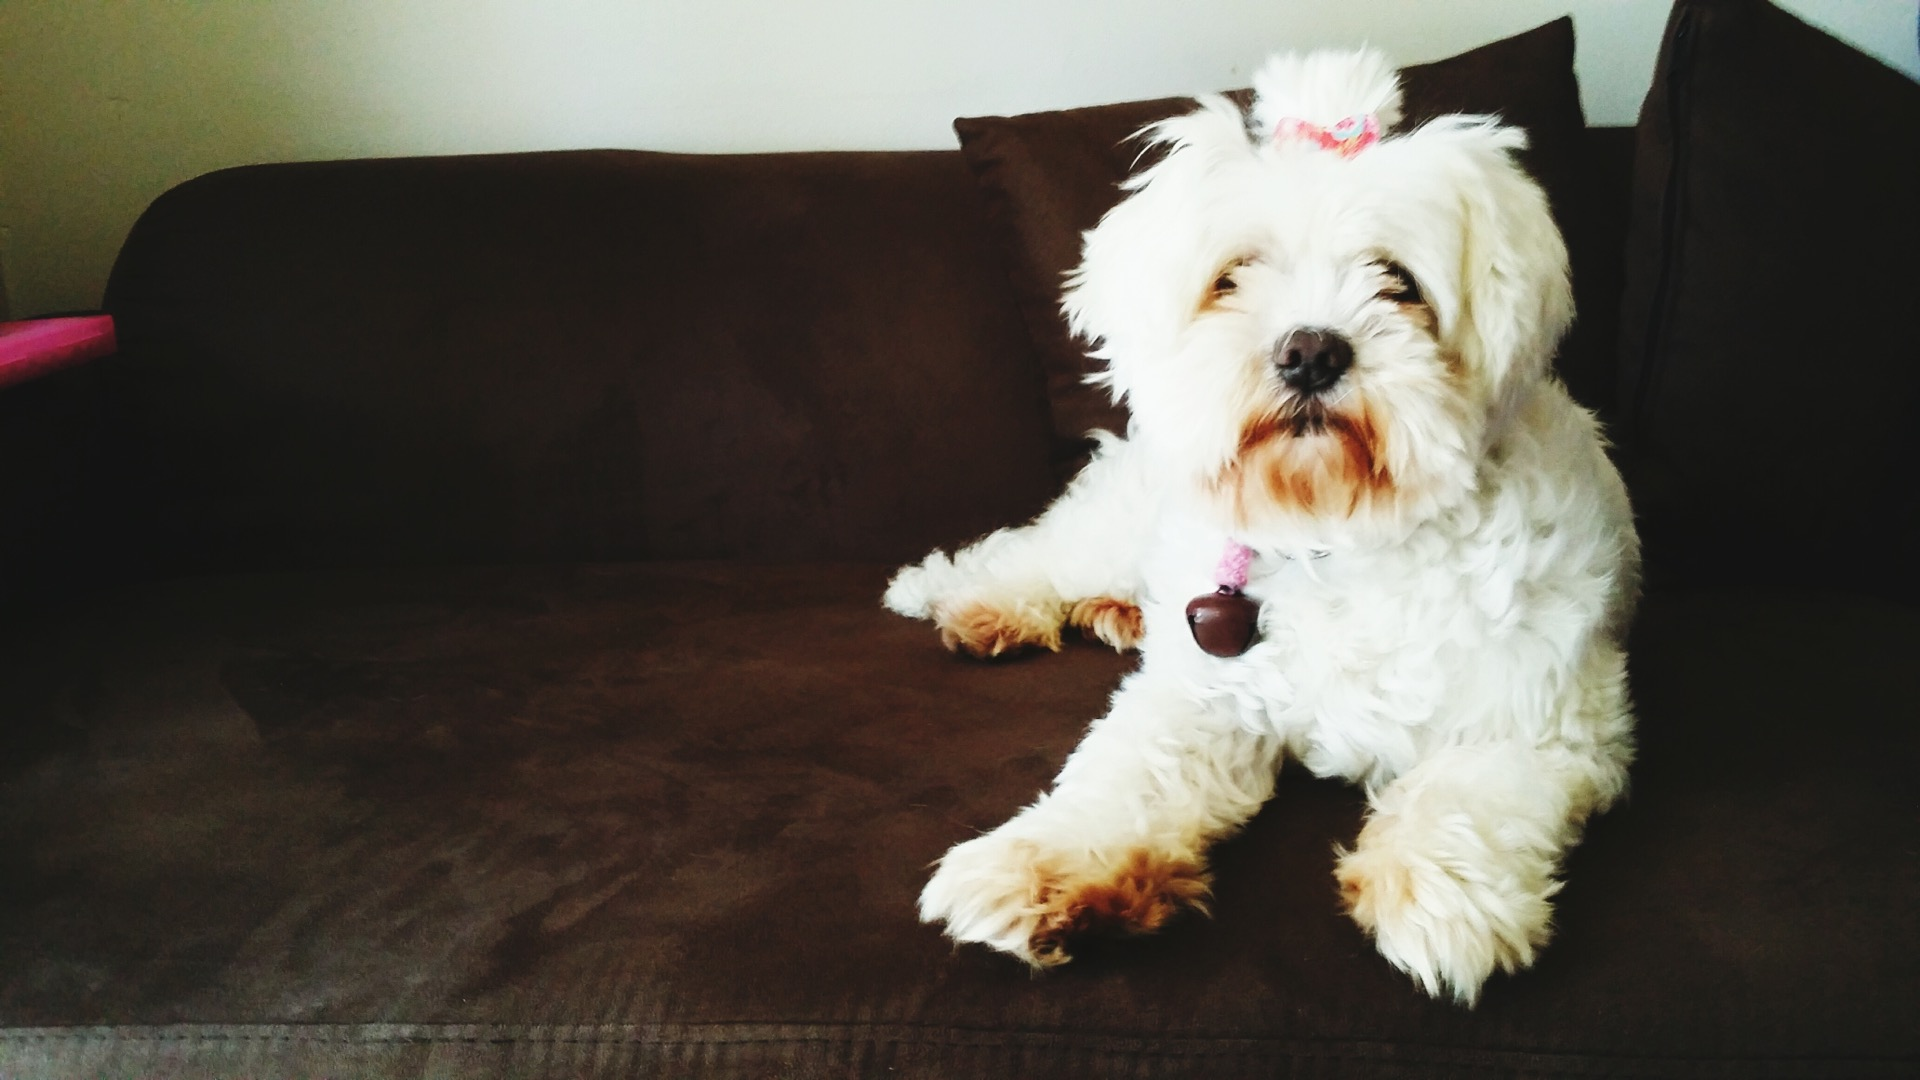
\includegraphics[height=3cm]{ex_29_img_1.png}
        \caption{a white dog sitting on top of a brown couch}
        \end{subfigure}% 
        \caption*{\textit{Relation}}
    \end{minipage}
    \hfill
    \begin{minipage}[t]{.30\textwidth}
        \begin{subfigure}[t]{\textwidth}
        \centering
        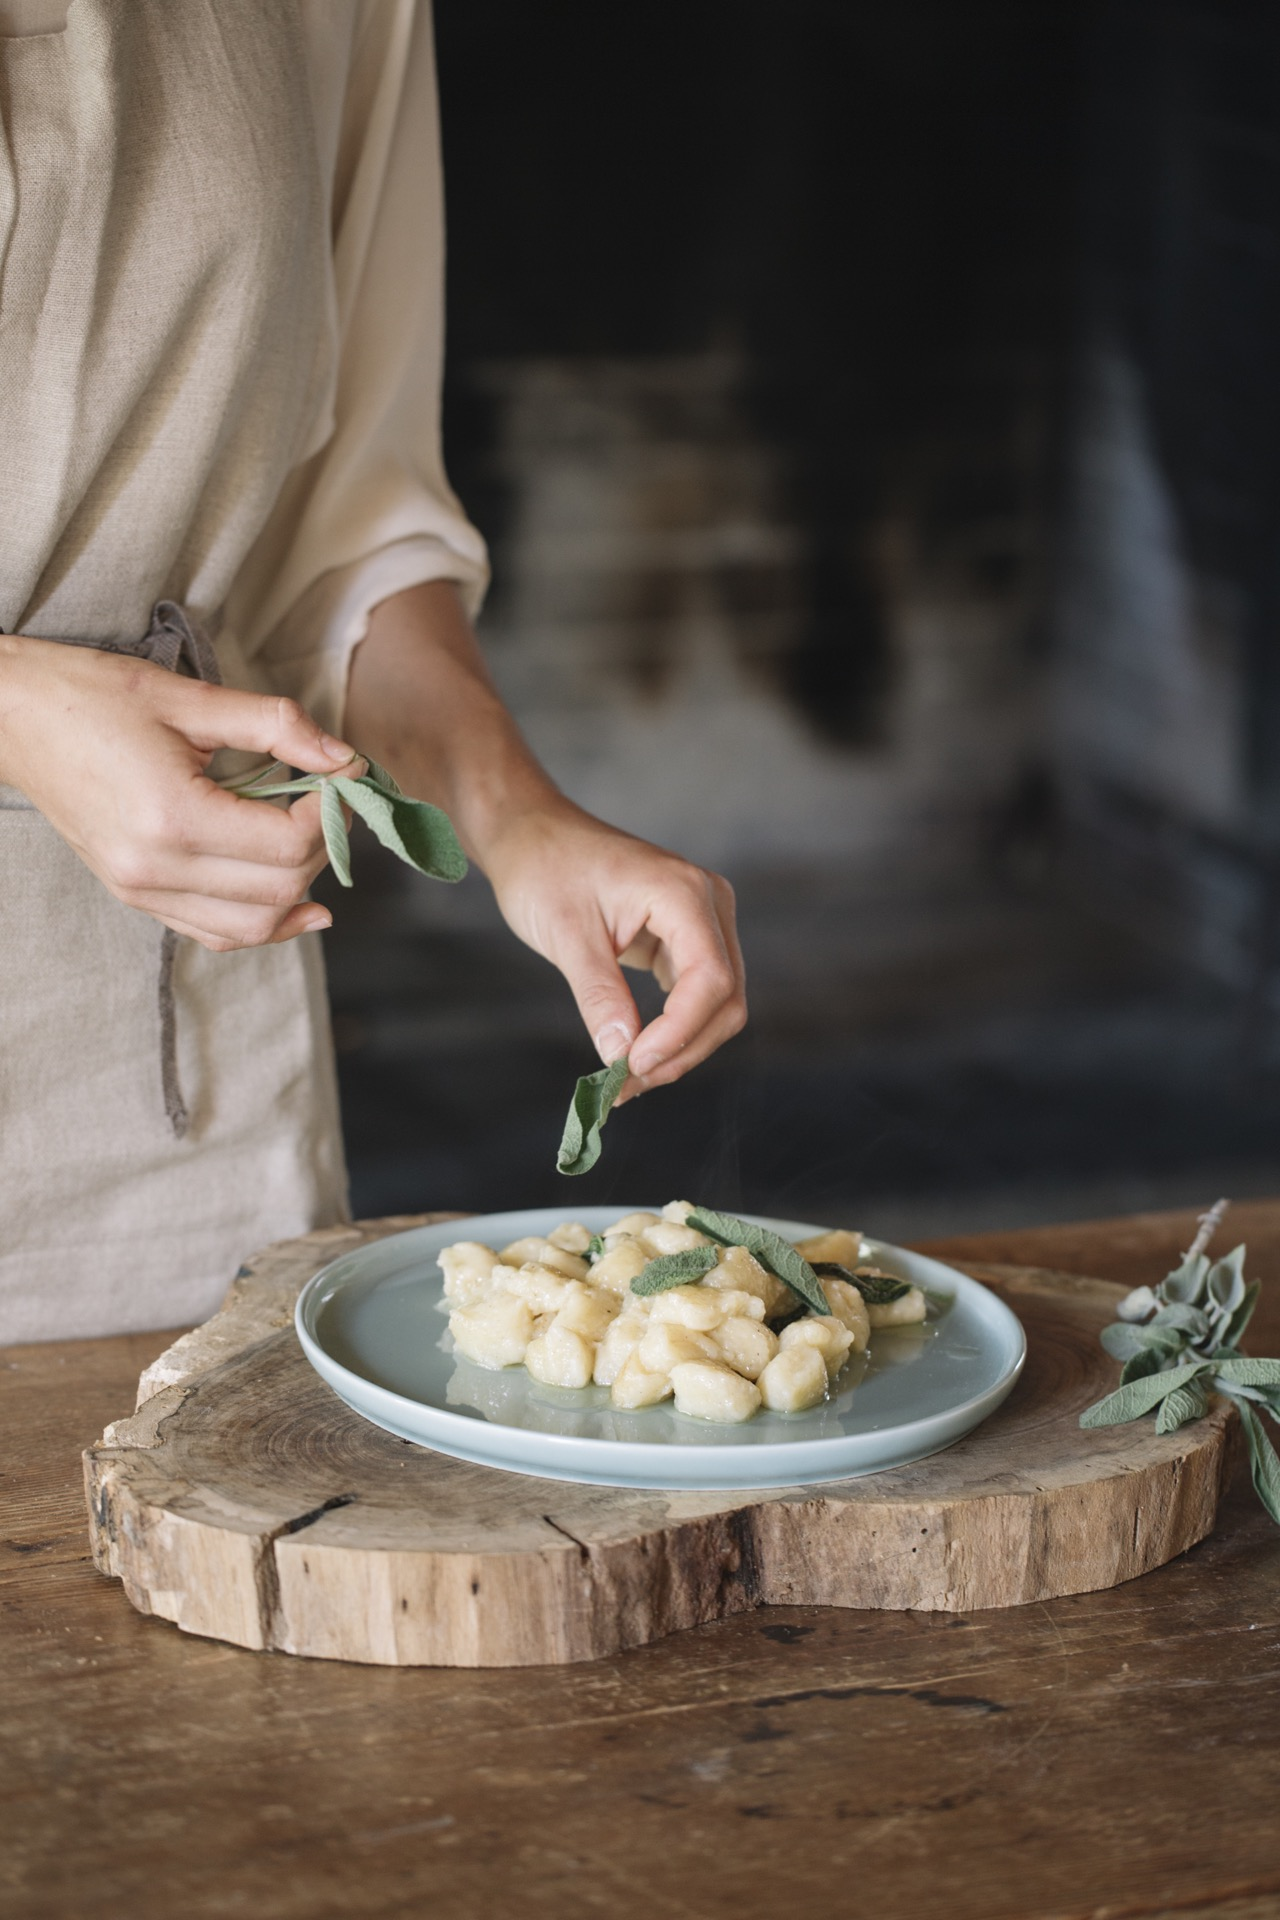
\includegraphics[height=3cm]{ex_118_img_0.png}
        \caption{a woman sprinkling herbs on a plate of food}
        \end{subfigure}\\
        \begin{subfigure}[t]{\textwidth}
        \centering
        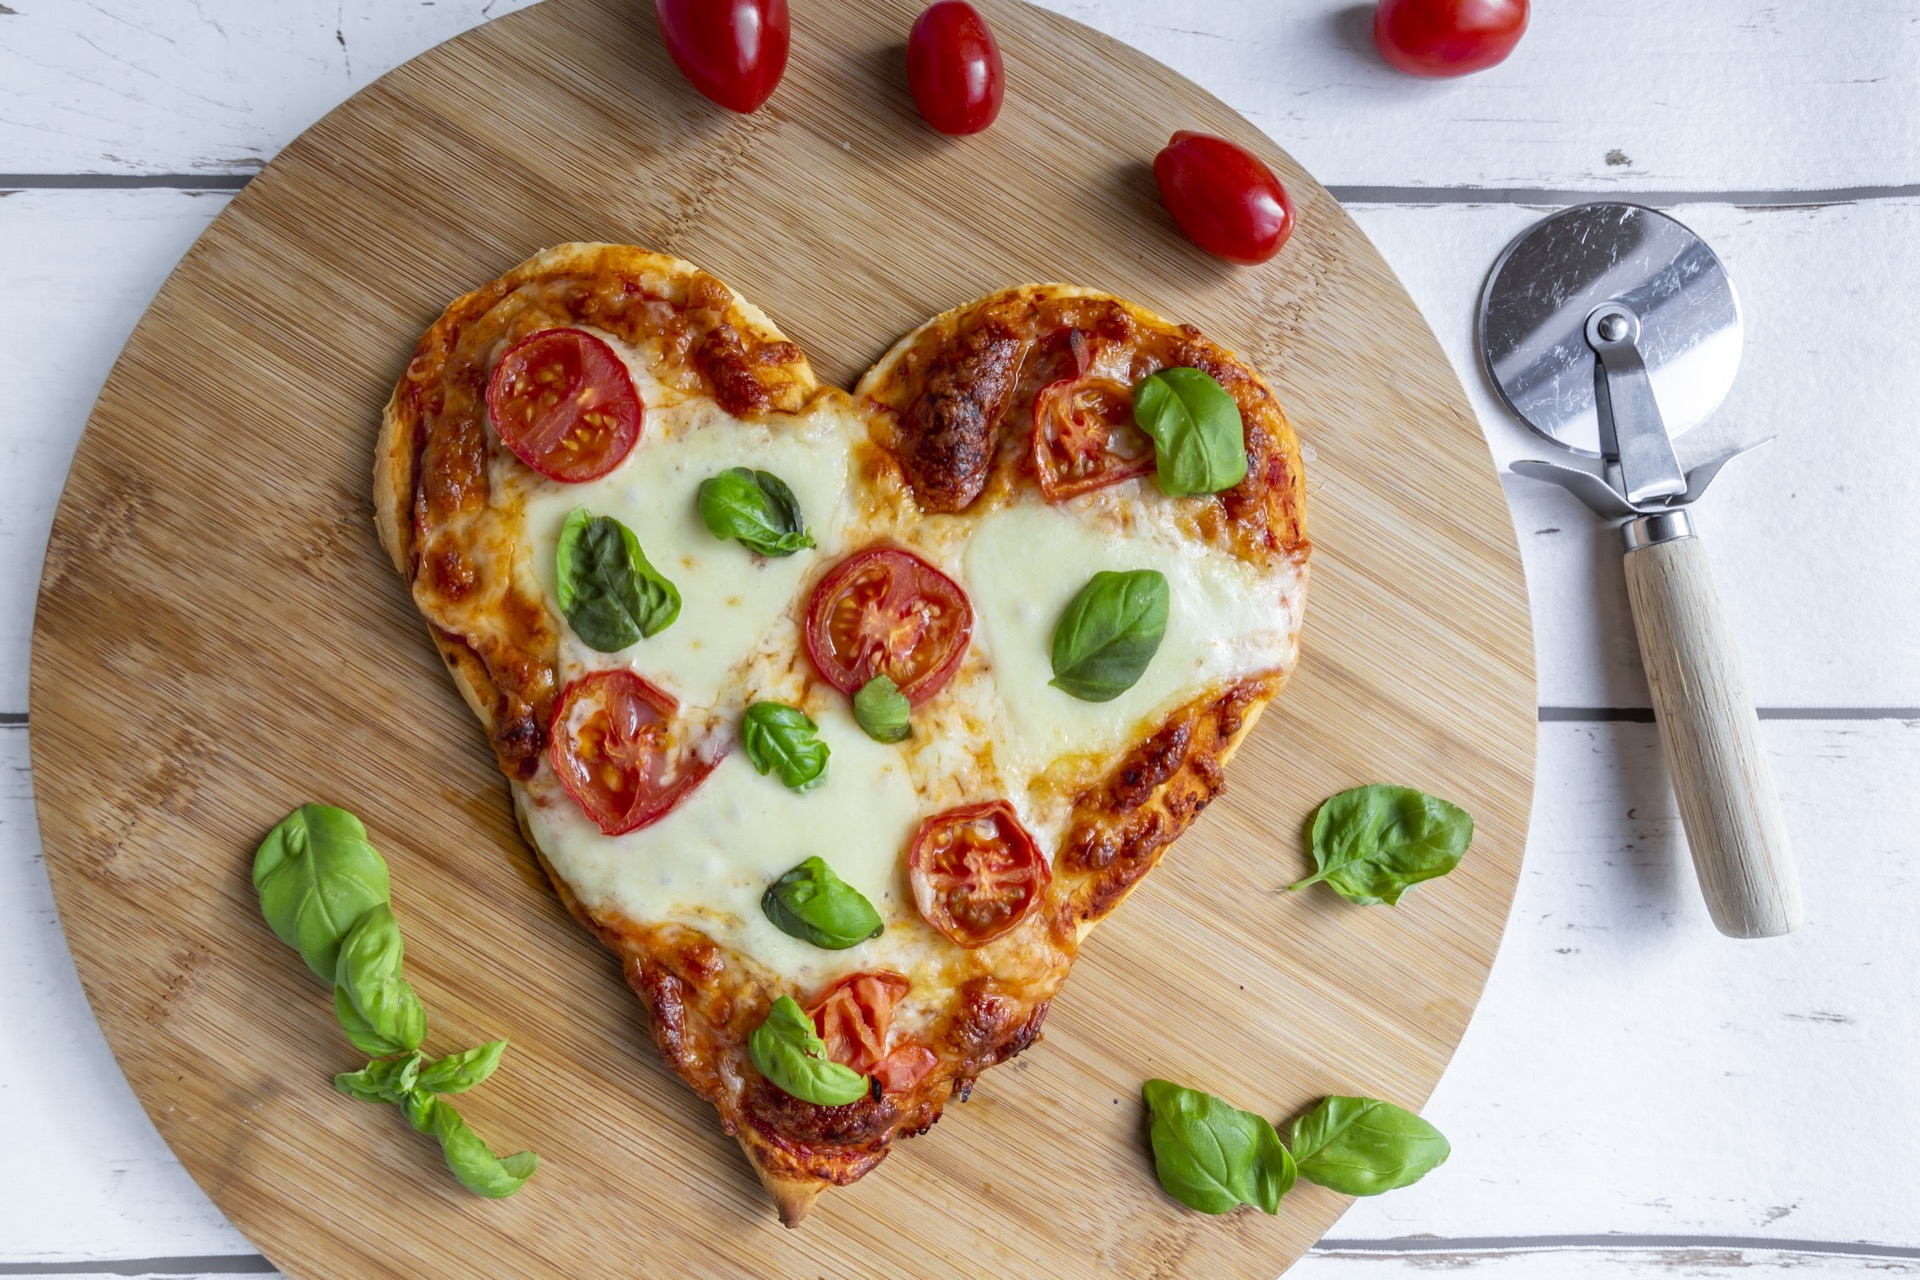
\includegraphics[height=3cm]{ex_118_img_1.png}
        \caption{a heart shaped pizza sitting on top of a cutting board}
        \end{subfigure}%
        \caption*{\textit{Relation}}
    \end{minipage}%
    \caption{Image Captioning examples from the Winoground dataset for the swap-dependent linguistic tags \textit{Object}, \textit{Relation} and \textit{Relation} from left to right. They are additionally tagged with 1 main predicate.}
    \label{fig:captioning-examples}
\end{figure}

Every caption in \cref{fig:captioning-examples-linguistic} is also correct. However, some important details that are present in the original captions are missing. In the second pair of images, the first caption does not mention the person, and the second one does not specify that the dog is sitting.

\begin{figure}[ht]
\centering
    \begin{minipage}[t]{.30\textwidth}
        \begin{subfigure}[t]{\textwidth}
        \centering
        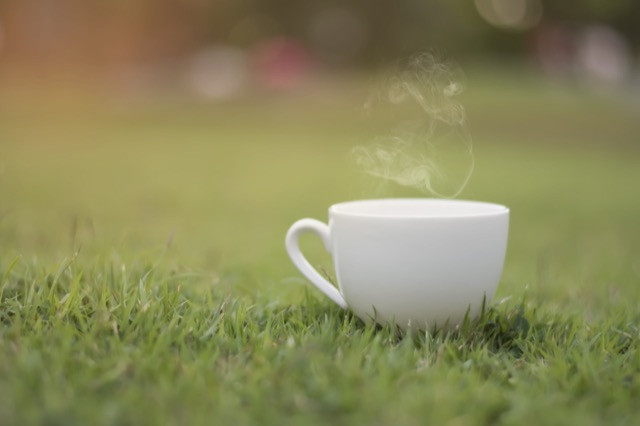
\includegraphics[height=3cm]{ex_14_img_0.png}
        \caption{a cup of coffee sitting on top of a lush green field}
        \end{subfigure}\\
        \begin{subfigure}[t]{\textwidth}
        \centering
        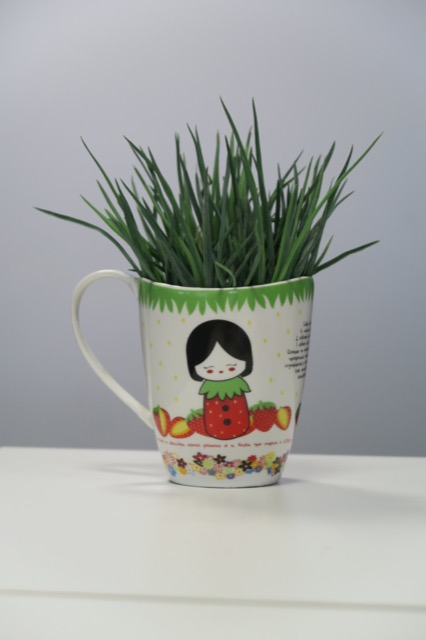
\includegraphics[height=3cm]{ex_14_img_1.png}
        \caption{a cup with a plant in it sitting on a table}
        \end{subfigure}%    
        \caption*{\textit{Object}}
    \end{minipage}
    \hfill
    \begin{minipage}[t]{.30\textwidth}
        \begin{subfigure}[t]{\textwidth}
        \centering
        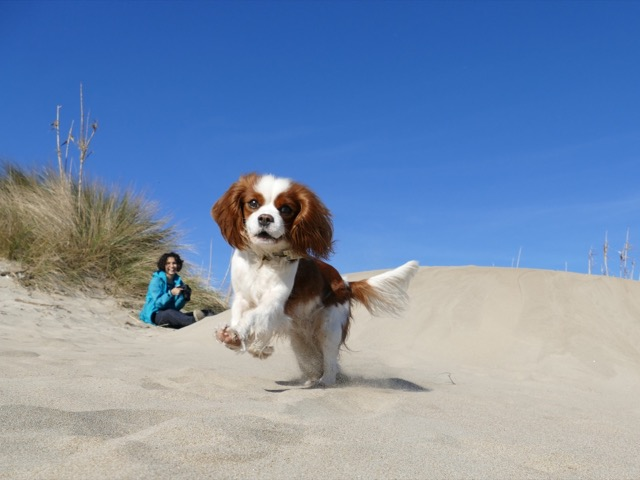
\includegraphics[height=3cm]{ex_21_img_0.png}
        \caption{a brown and white dog running in the sand}
        \end{subfigure}\\
        \begin{subfigure}[t]{\textwidth}
        \centering
        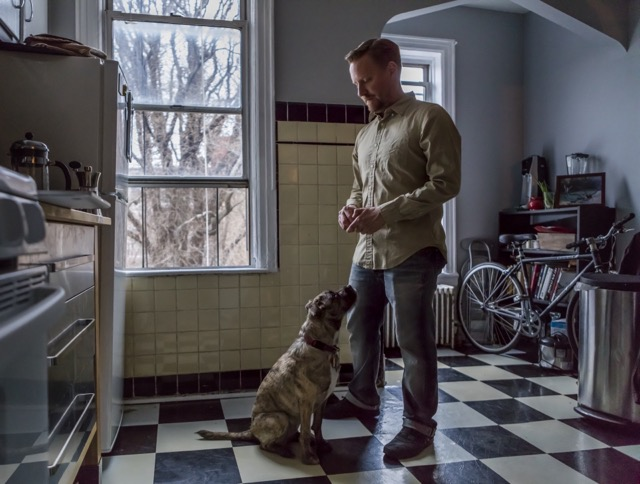
\includegraphics[height=3cm]{ex_21_img_1.png}
        \caption{a man standing next to a dog in a kitchen}
        \end{subfigure}%    
        \caption*{\textit{Relation}}
    \end{minipage}
    \hfill
    \begin{minipage}[t]{.30\textwidth}
        \begin{subfigure}[t]{\textwidth}
        \centering
        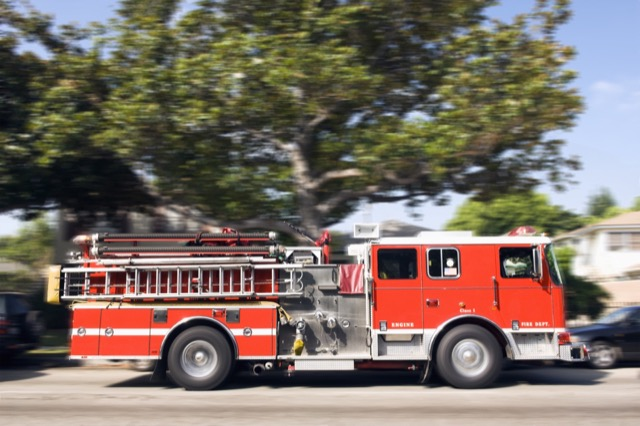
\includegraphics[height=3cm]{ex_72_img_0.png}
        \caption{a red fire truck driving down a street}
        \end{subfigure}\\
        \begin{subfigure}[t]{\textwidth}
        \centering
        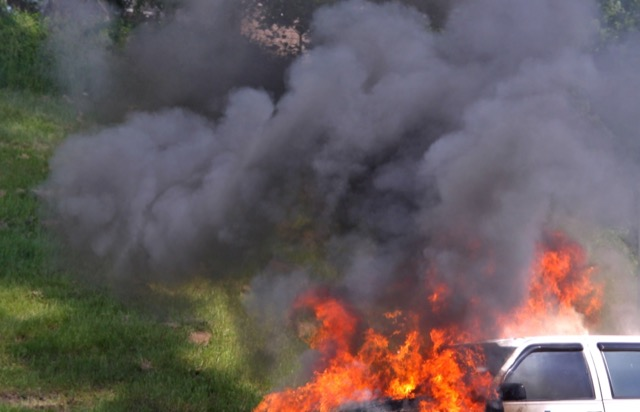
\includegraphics[height=3cm]{ex_72_img_1.png}
        \caption{a car is on fire in a field}
        \end{subfigure}%
        \vspace{10pt}
        \caption*{\textit{Both}}
    \end{minipage}%
    \caption{Image Captioning examples from the Winoground dataset for the swap-dependent linguistic tags \textit{Object}, \textit{Relation} and \textit{Both} from left to right. They are additionally tagged with 1, 2 and 1 main predicates from left to right.}
    \label{fig:captioning-examples-linguistic}
\end{figure}

The first pair of captions in \cref{fig:captioning-examples-visual} is wrong. In the first image, the young boy is the one holding the magnifying glass. The second one is completely wrong, they are not sitting at a table and the magnifying glass is not mentioned. Other examples are correct, but more generic than the original captions. The describe the images, without mentioning detains such as the number of people and windows.

\begin{figure}[ht]
\centering
    \begin{minipage}{.30\textwidth}
        \begin{subfigure}{\textwidth}
        \centering
        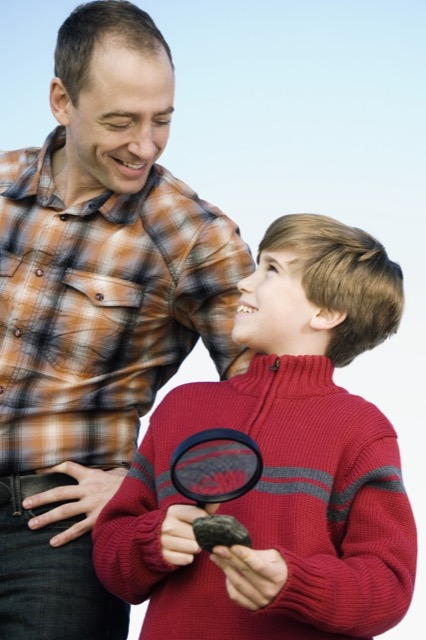
\includegraphics[height=3cm]{ex_75_img_0.png}
        \caption{a man holding a magnifying glass next to a young boy}
        \end{subfigure}\\
        \begin{subfigure}{\textwidth}
        \centering
        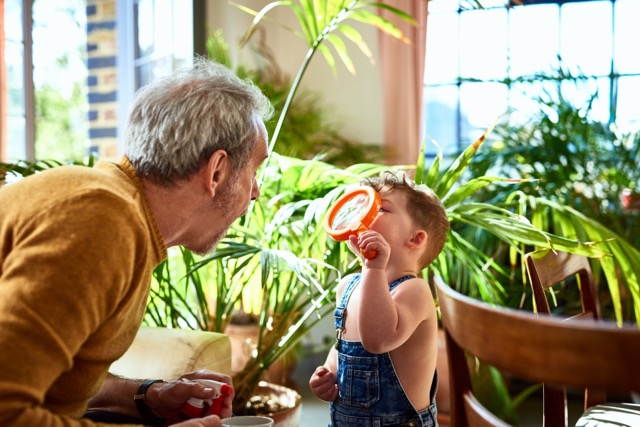
\includegraphics[height=3cm]{ex_75_img_1.png}
        \caption{a man and a little girl sitting at a table}
        \end{subfigure}%    
        \caption*{\textit{Pragmatics}}
    \end{minipage}
    \hfill
    \begin{minipage}{.30\textwidth}
        \begin{subfigure}{\textwidth}
        \centering
        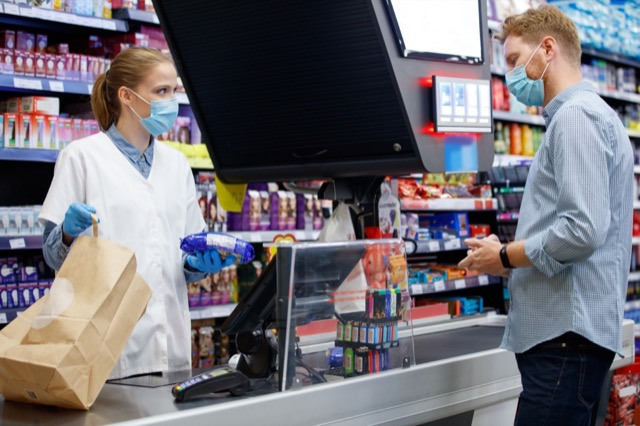
\includegraphics[height=3cm]{ex_27_img_0.png}
        \caption{a man and a woman wearing face masks in a store}
        \end{subfigure}\\
        \begin{subfigure}{\textwidth}
        \centering
        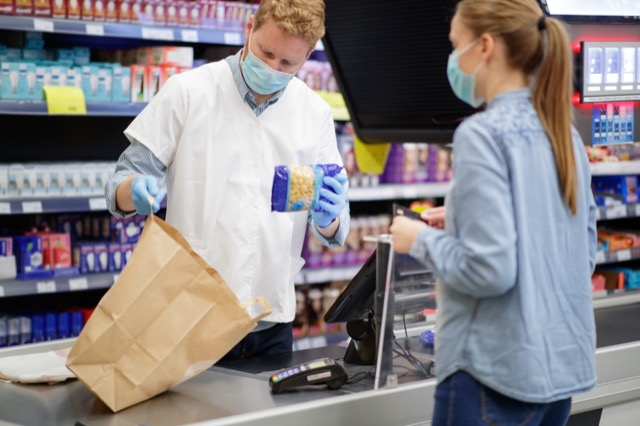
\includegraphics[height=3cm]{ex_27_img_1.png}
        \caption{a man and a woman in a grocery store}
        \end{subfigure}%    
        \caption*{\textit{Series}}
    \end{minipage}
    \hfill
    \begin{minipage}{.30\textwidth}
        \begin{subfigure}{\textwidth}
        \centering
        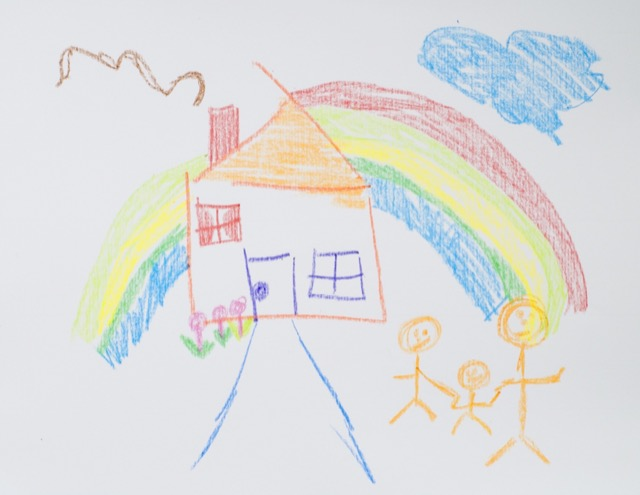
\includegraphics[height=3cm]{ex_61_img_0.png}
        \caption{a child's drawing of a house with a rainbow}
        \end{subfigure}\\
        \begin{subfigure}{\textwidth}
        \centering
        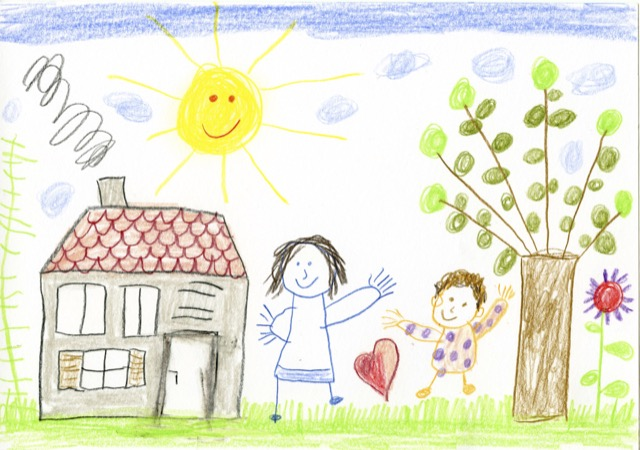
\includegraphics[height=3cm]{ex_61_img_1.png}
        \caption{a child's drawing of a house and a girl}
        \end{subfigure}%    
        \caption*{\textit{Symbolic}}
    \end{minipage}
    \caption{Image Captioning examples from the Winoground dataset for the visual tags \textit{Pragmatics}, \textit{Series} and \textit{Symbolic} from left to right. They are additionally tagged with the \textit{Relation} tag, and 1, 2, and 1 main predicate from left to right.}
    \label{fig:captioning-examples-visual}
\end{figure}

The general conclusion is that most captions are quite good. They are very different from the original ones, but they describe the images correctly. They provide extra information about the images to the models, that is not included in the original captions. They could be used to improve the results of the models by incorporating them into the evaluation process. For example, we could compare the original and generated captions and pair them by similarity. 

Captioning could also be applied for generating automatic descriptions of images. This would reduce the work needed to create training datasets targeted for compositional or spatial reasoning.

It seems that these models are not that bad at describing images, but have more difficulties when pairing them with very similar captions. This suggests that text encoding might be their biggest limitation, and could be the main reason for their low performance on Winoground.

\section{Image Retrieval} \label{sec:image_retrieval}

We used CLIP retrieval\footnote{\url{https://github.com/rom1504/clip-retrieval}} to retrieve images from LAION-5B \cite{schuhmann2022laionb} dataset. We used Winoground captions and images to get similar images. For each caption and image, we compute its embeddings using CLIP ViT-L-14. Then the system uses a KNN algorithm to retrieve images that have similar embeddings. We can also compute the mean of caption and image embeddings to retrieve images that match both the image and the caption. 

We used the python CLIP Client with the default parameters, which retrieves a maximum of 40 images with each query. It also retrieves the original caption of the image and a similarity score. The system also has an aesthetic score that can be used to retrieve better looking images. It also removes duplicate images and images that contain unsafe content and violence. \cref{fig:retrieval_interface} shows an example search with the alternative retrieval interface\footnote{\url{https://rom1504.github.io/clip-retrieval}}.

\begin{figure}[ht]
    \centering
    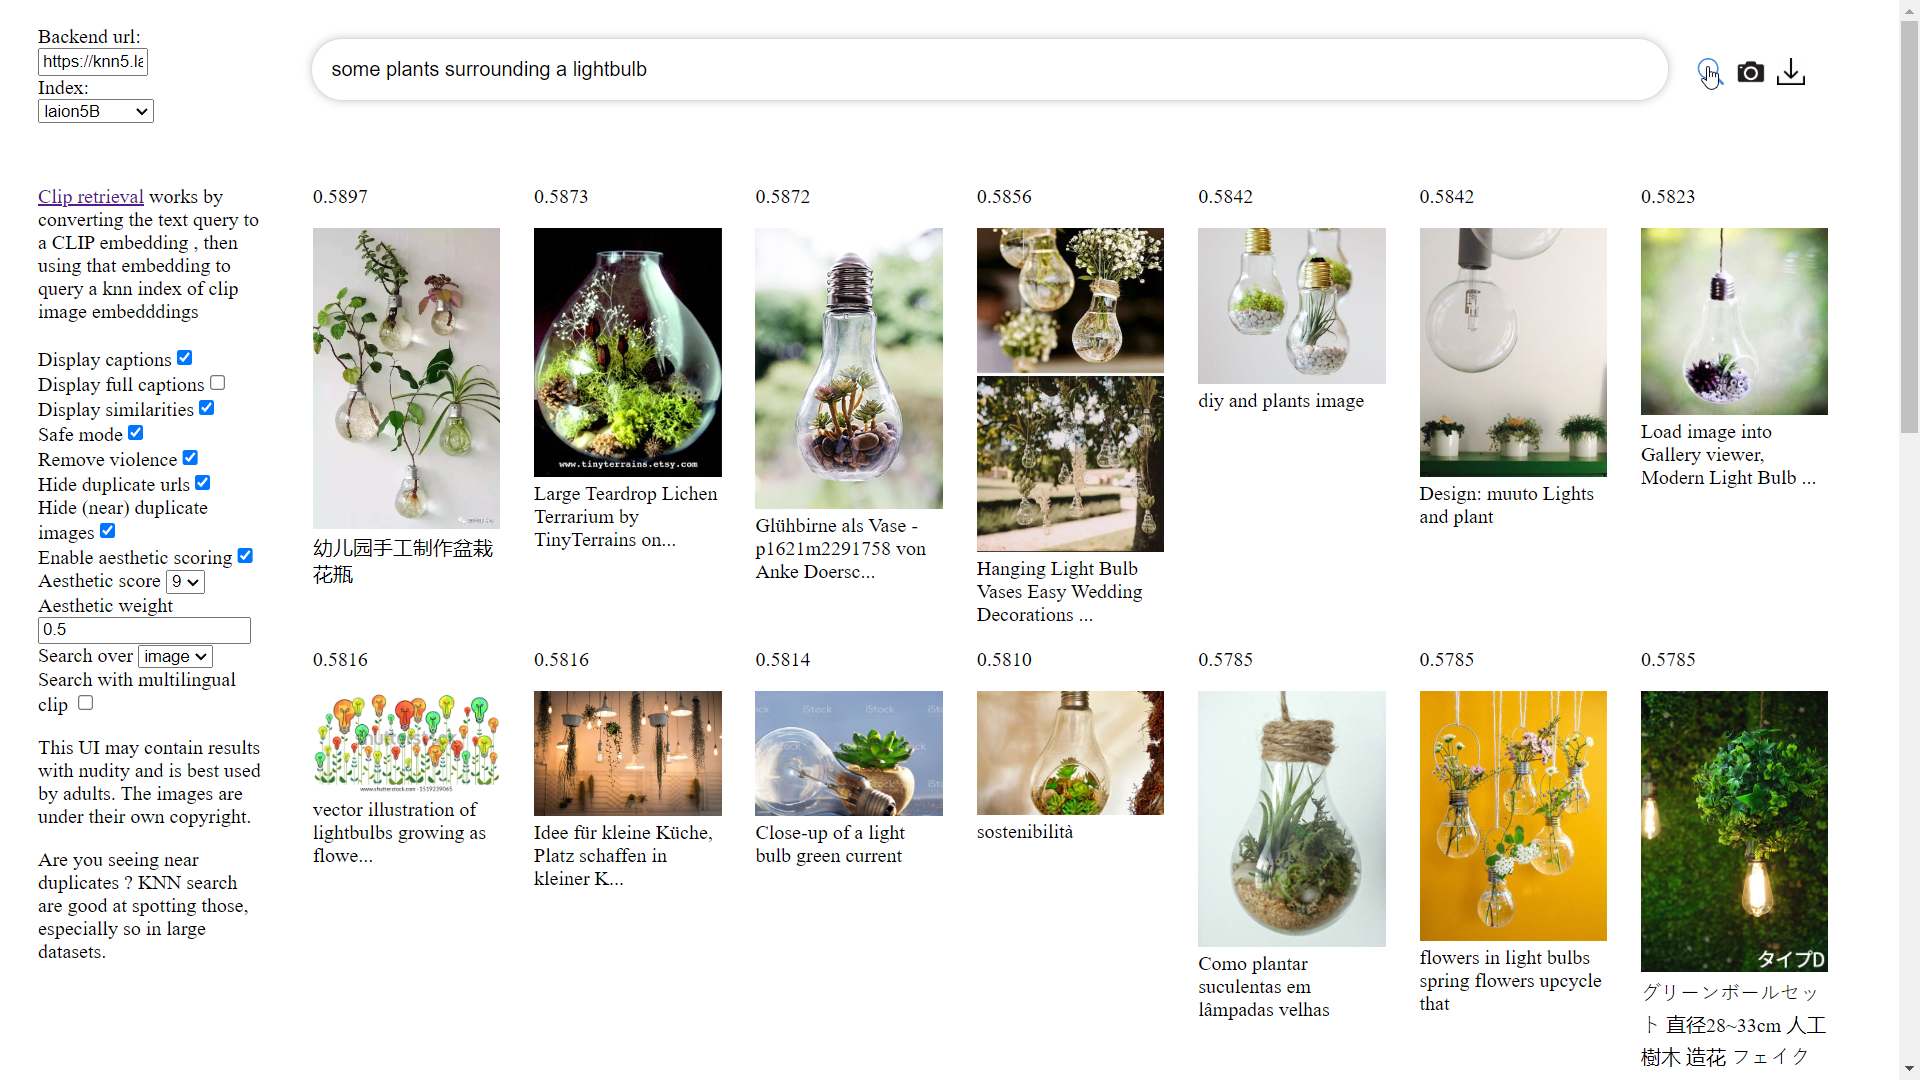
\includegraphics[width=\linewidth]{retrieval/interface.png}
    \caption{CLIP Retrieval interface search example. Many of the images are wrong and correspond to the other caption.}
    \label{fig:retrieval_interface}
\end{figure}

We have selected a few examples of retrieved images to compare them with the original images. These images were retrieved using only the captions. Only the first generated image is shown in the examples, which is not necessarily the best one. The complete retrieval file can be found in the GitHub repository.

In \cref{fig:retrieval-examples}, the first pair of images is correct, both images match the captions. In the second pair, the color of the dog is correct, but the couch has a wrong color. In the third example, the first image has wrong shapes and the second image is wrong.

\begin{figure}[ht]
\centering
    \begin{minipage}[t]{.30\textwidth}
        \begin{subfigure}[t]{\textwidth}
        \centering
        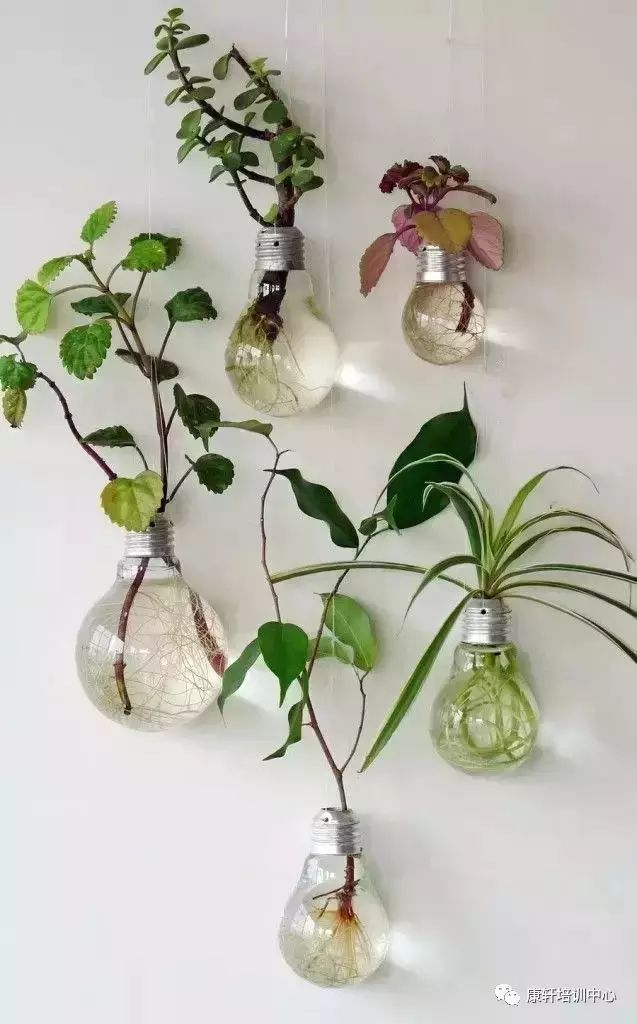
\includegraphics[height=3cm]{retrieval/ex_155_cap_0_img_0.jpg}
        \caption{[some plants] surrounding [a lightbulb]}
        \end{subfigure}\\
        \begin{subfigure}[t]{\textwidth}
        \centering
        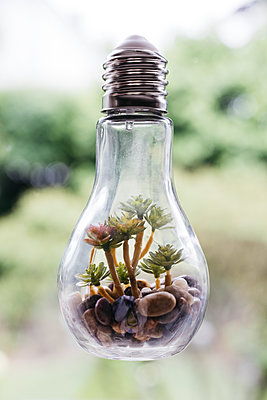
\includegraphics[height=3cm]{retrieval/ex_155_cap_1_img_0.jpg}
        \caption{[a lightbulb] surrounding [some plants]}
        \end{subfigure}%
        \caption*{\textit{Object}}
    \end{minipage}
    \hfill
    \begin{minipage}[t]{.30\textwidth}
        \begin{subfigure}[t]{\textwidth}
        \centering
        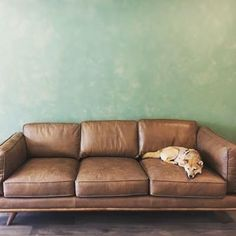
\includegraphics[height=3cm]{retrieval/ex_29_cap_0_img_0.jpg}
        \caption{a [brown] dog is on a [white] couch}
        \end{subfigure}\\
        \vspace{10pt}
        \begin{subfigure}[t]{\textwidth}
        \centering
        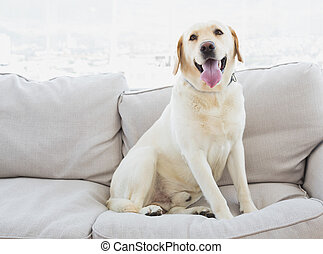
\includegraphics[height=3cm]{retrieval/ex_29_cap_1_img_0.jpg}
        \caption{a [white] dog is on a [brown] couch}
        \end{subfigure}%
        \vspace{10pt}
        \caption*{\textit{Relation}}
    \end{minipage}
    \hfill
    \begin{minipage}[t]{.30\textwidth}
        \begin{subfigure}[t]{\textwidth}
        \centering
        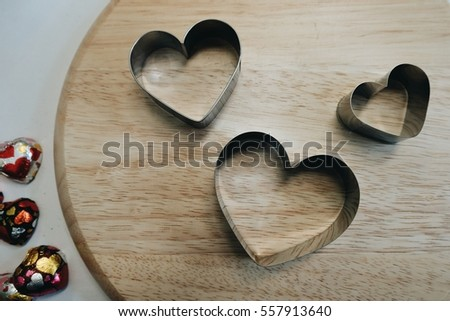
\includegraphics[height=3cm]{retrieval/ex_118_cap_0_img_0.jpg}
        \caption{[circular] food on [heart-shaped] wood}
        \end{subfigure}\\
        \begin{subfigure}[t]{\textwidth}
        \centering
        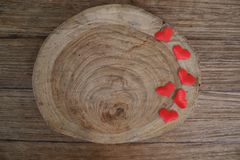
\includegraphics[height=3cm]{retrieval/ex_118_cap_1_img_0.jpg}
        \caption{[heart-shaped] food on [circular] wood}
        \end{subfigure}%
        \caption*{\textit{Relation}}
    \end{minipage}%
    \caption{CLIP Retrieval examples for the swap-dependent linguistic tags \textit{Object}, \textit{Relation} and \textit{Relation} from left to right. The linguistic examples are additionally tagged with 1 main predicate.}
    \label{fig:retrieval-examples}
\end{figure}

In \cref{fig:retrieval-examples-linguistic}, the first pair is correct. The second pair is wrong, the same image is retrieved for both captions. The first image in the third example is correct, but the second one is incorrect.

\begin{figure}[ht]
\centering
    \begin{minipage}[t]{.30\textwidth}
        \begin{subfigure}[t]{\textwidth}
        \centering
        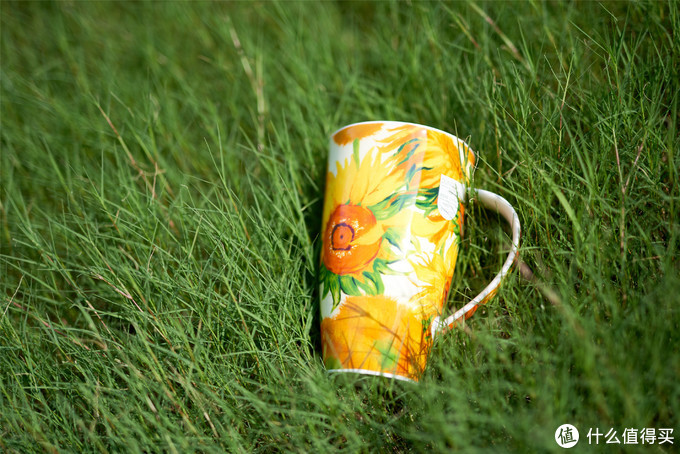
\includegraphics[height=3cm]{retrieval/ex_14_cap_0_img_0.jpg}
        \caption{there is [a mug] in [some grass]}
        \end{subfigure}\\
        \begin{subfigure}[t]{\textwidth}
        \centering
        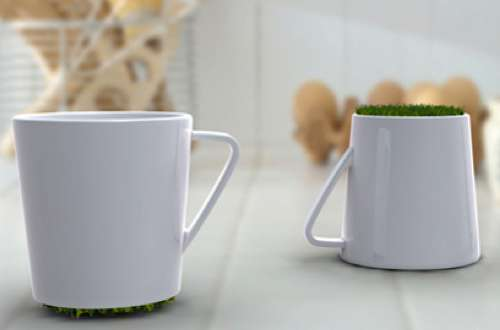
\includegraphics[height=3cm]{retrieval/ex_14_cap_1_img_0.jpg}
        \caption{there is [some grass] in [a mug]}
        \end{subfigure}%    
        \caption*{\textit{Object}}
    \end{minipage}
    \hfill
    \begin{minipage}[t]{.30\textwidth}
        \begin{subfigure}[t]{\textwidth}
        \centering
        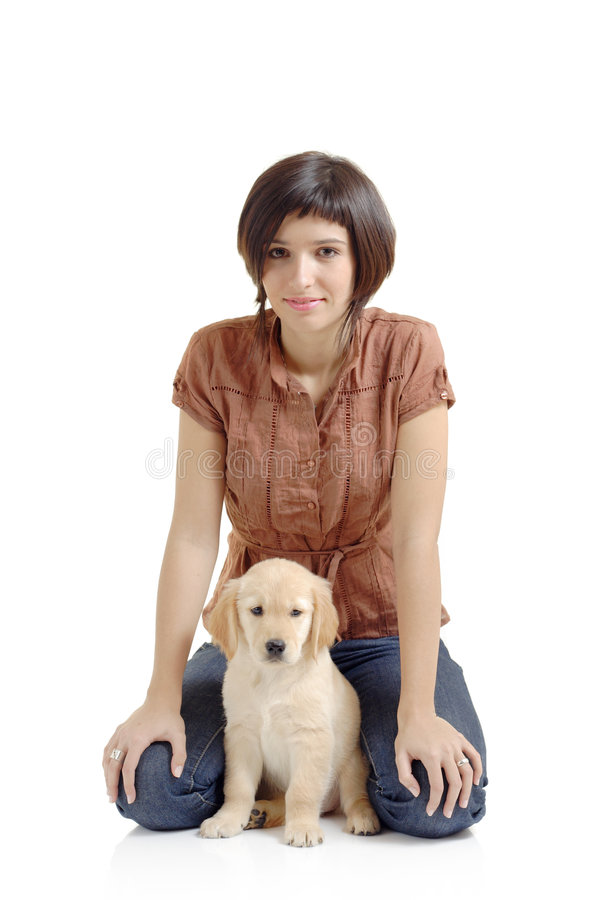
\includegraphics[height=3cm]{retrieval/ex_21_cap_0_img_0.jpg}
        \caption{a person [sits] and a dog [stands]}
        \end{subfigure}\\
        \begin{subfigure}[t]{\textwidth}
        \centering
        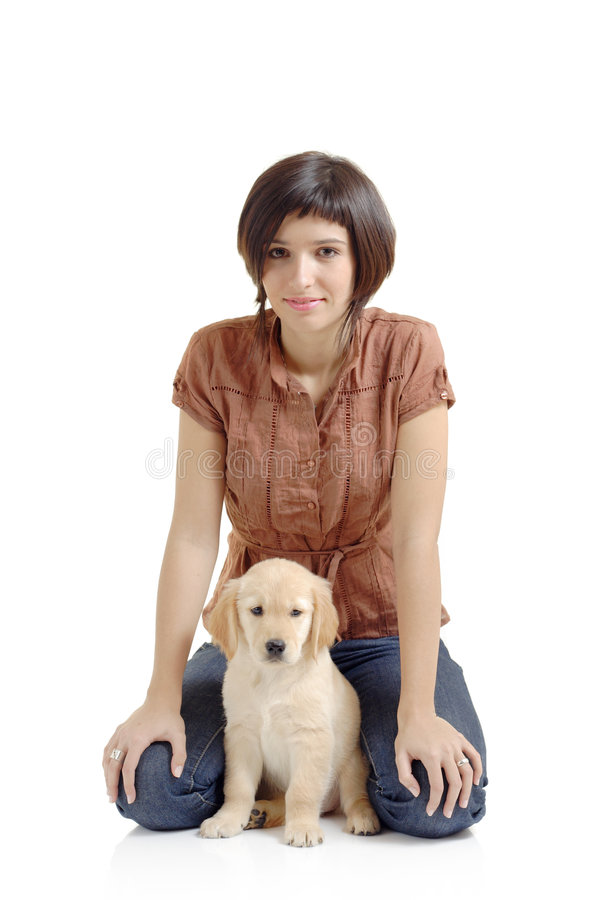
\includegraphics[height=3cm]{retrieval/ex_21_cap_1_img_0.jpg}
        \caption{a person [stands] and a dog [sits]}
        \end{subfigure}%    
        \caption*{\textit{Relation}}
    \end{minipage}
    \hfill
    \begin{minipage}[t]{.30\textwidth}
        \begin{subfigure}[t]{\textwidth}
        \centering
        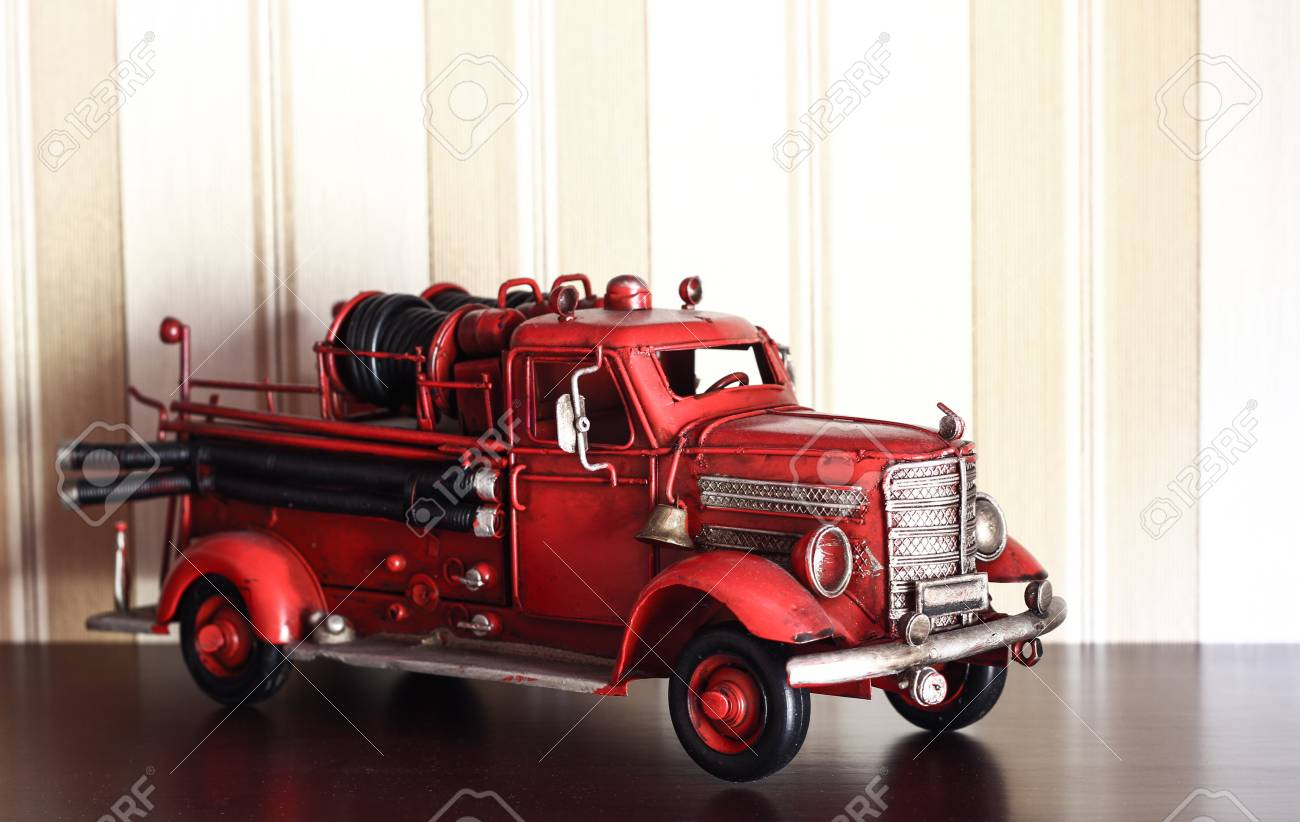
\includegraphics[height=3cm]{retrieval/ex_72_cap_0_img_0.jpg}
        \caption{it's a [fire] [truck]}
        \end{subfigure}\\
        \begin{subfigure}[t]{\textwidth}
        \centering
        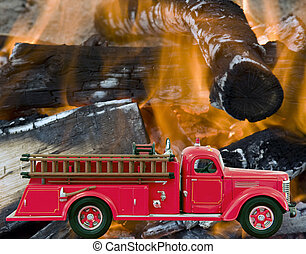
\includegraphics[height=3cm]{retrieval/ex_72_cap_1_img_0.jpg}
        \caption{it's a [truck] [fire]}
        \end{subfigure}%
        \caption*{\textit{Both}}
    \end{minipage}%
    \caption{CLIP Retrieval examples for the swap-dependent linguistic tags \textit{Object}, \textit{Relation} and \textit{Both} from left to right. The linguistic examples are additionally tagged with 1, 2 and 1 main predicates from left to right.}
    \label{fig:retrieval-examples-linguistic}
\end{figure}

In \cref{fig:retrieval-examples-visual}, the first example is wrong, the objects are present but the composition is not correct. In the second pair, some objects are missing in both images. The third pair is wrong, the same image is retrieved, which only contains two windows and no people.

\begin{figure}[ht]
\centering
    \begin{minipage}{.30\textwidth}
        \begin{subfigure}{\textwidth}
        \centering
        \includegraphics[height=3cm]{retrieval/ex_75_cap_0_img_0.jpg}
        \caption{the kid [with the magnifying glass] looks at them []}
        \end{subfigure}\\
        \begin{subfigure}{\textwidth}
        \centering
        \includegraphics[height=3cm]{retrieval/ex_75_cap_1_img_0.jpg}
        \caption{the kid [] looks at them [with the magnifying glass]}
        \end{subfigure}%    
        \caption*{\textit{Pragmatics}}
    \end{minipage}
    \hfill
    \begin{minipage}{.30\textwidth}
        \begin{subfigure}{\textwidth}
        \centering
        \includegraphics[height=3cm]{retrieval/ex_27_cap_0_img_0.jpg}
        \caption{the person with the ponytail [packs] stuff and other [buys] it}
        \end{subfigure}\\
        \begin{subfigure}{\textwidth}
        \centering
        \includegraphics[height=3cm]{retrieval/ex_27_cap_1_img_0.jpg}
        \caption{the person with the ponytail [buys] stuff and other [packs] it}
        \end{subfigure}%    
        \caption*{\textit{Series}}
    \end{minipage}
    \hfill
    \begin{minipage}{.30\textwidth}
        \begin{subfigure}{\textwidth}
        \centering
        \includegraphics[height=3cm]{retrieval/ex_61_cap_0_img_0.jpg}
        \caption{there are [three] people and [two] windows}
        \end{subfigure}\\
        \begin{subfigure}{\textwidth}
        \centering
        \includegraphics[height=3cm]{retrieval/ex_61_cap_1_img_0.jpg}
        \caption{there are [two] people and [three] windows}
        \end{subfigure}%    
        \caption*{\textit{Symbolic}}
    \end{minipage}
    \caption{CLIP Retrieval examples for the visual tags \textit{Pragmatics}, \textit{Series} and \textit{Symbolic} from left to right. The visual examples are additionally tagged with the \textit{Relation} tag, and 1, 2, and 1 main predicates from left to right.}
    \label{fig:retrieval-examples-visual}
\end{figure}

This system could be used to increase the size of our dataset. We could retrieve many similar images for our captions. We could also change the captions to retrieve images with different objects. Nevertheless, this would also require some filtering because there are many wrong images.

The number of retrieved images and the similarity score could also be used as a measure of how common an image is. If there are very few similar images in the dataset, that means that the caption or image is uncommon. However, the system might not be robust enough for this estimation.